% Chapter 3

\chapter{Methodology}

\label{Chapter3} % For referencing the chapter elsewhere, use \ref{Chapter3} 

The development of this personalized learning platform involved integrating advanced technologies and APIs to deliver an interactive and customized learning experience. The methodology comprises several key steps, each designed to ensure seamless functionality and robust performance. The technologies utilized include Next.js, OpenAI GPT models, YouTube API, Unsplash API, and LangChain. Below is a detailed explanation of the workflow:

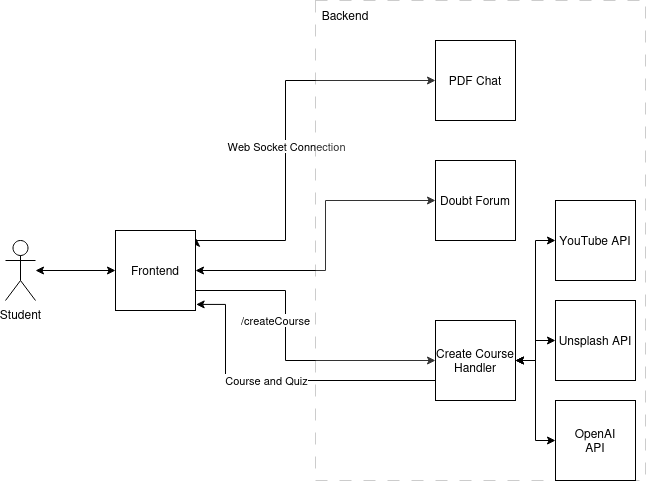
\includegraphics[scale=0.55]{Images/7th sem major project.drawio.png}
\section{Course Content Creation}
The learning process begins with the user creating a course entry. The user specifies the title of the course and its subunits (e.g., chapters or modules). This step allows users to define the basic structure of the course, ensuring flexibility in tailoring the content to their needs. For example, a user preparing for a "Machine Learning" course may create subunits such as "Supervised Learning," "Unsupervised Learning," and "Neural Networks."

\section{Sending Data to OpenAI GPT Model}
Once the course structure is defined, the data is sent to the OpenAI GPT model. The model processes each subunit and generates a detailed breakdown of topics related to it. For instance, if the subunit is "Supervised Learning," the model may output topics such as "Linear Regression," "Decision Trees," and "Support Vector Machines." The result is returned as a JSON response, which contains:
\begin{itemize}
    \item Chapter or unit names
    \item YouTube search queries for each topic
    \item Quiz questions related to the topics
\end{itemize}

\section{YouTube API Integration}
The JSON response from the GPT model is passed to a function that iterates through the generated topics and corresponding YouTube search queries. Using the YouTube API, the function fetches relevant educational videos for each topic. For example, if the query is "Linear Regression tutorial," the API retrieves high-quality video resources that are displayed on the frontend. This integration ensures that users have access to curated video content that aligns with their learning objectives.

\section{Quiz Generation}
The GPT model also generates quick quizzes for each topic. These quizzes are designed to reinforce the user's understanding of the material by testing their knowledge in a focused and interactive manner. For example, a quiz for "Decision Trees" might include questions like:
\begin{quote}
    "What is the purpose of splitting criteria in a decision tree?"
\end{quote}
The quizzes are dynamically created, providing immediate feedback to users.

\section{Chat with PDF Functionality}
In addition to video-based learning, the platform incorporates a "Chat with PDF" feature powered by LangChain. Users can upload PDF notes or slides and interact with the document through natural language queries. For instance, a student studying "Calculus" can upload their lecture notes and ask questions like:
\begin{quote}
    "Can you explain the derivation of the chain rule?"
\end{quote}
This feature enables efficient self-study by transforming static resources into dynamic learning tools.

\section{Doubt Forum}
To foster collaborative learning, the platform includes a doubt forum. This feature allows users to post questions, seek clarification, and participate in discussions with peers and mentors. For example, a user might post a query about the application of "Gradient Descent in Machine Learning," prompting others to share explanations, resources, or experiences. The doubt forum creates a community-driven ecosystem that enhances the learning experience.

\section{Technologies Used}
The implementation of the platform relies on the following technologies:
\begin{itemize}
    \item \textbf{Next.js}: Used for developing a responsive and dynamic frontend.
    \item \textbf{OpenAI GPT Models}: Power the generation of course outlines, topics, and quizzes.
    \item \textbf{YouTube API}: Fetches relevant video resources for each topic.
    \item \textbf{Unsplash API}: Provides high-quality images to visually enrich the platform.
    \item \textbf{LangChain}: Enables the "Chat with PDF" functionality for text-based learning.
\end{itemize}

\section{Workflow Overview}
The complete workflow of the platform can be summarized as follows:
\begin{enumerate}
    \item User specifies the course title and subunits.
    \item Data is sent to OpenAI GPT, which generates topics, YouTube queries, and quiz questions.
    \item JSON responses are processed, and YouTube API calls are made to fetch relevant videos.
    \item The frontend displays the course outline, video recommendations, and quizzes.
    \item Users interact with PDF notes using the "Chat with PDF" feature.
    \item The doubt forum allows users to post and answer questions, creating a collaborative learning environment.
\end{enumerate}

This methodology ensures a comprehensive and seamless learning experience, combining AI-driven content generation with interactive and community-driven features.